\documentclass[UTF8,a4paper,11pt]{ctexart}

% T-23 v2 校赛内部复核稿：官方投稿模板尚未锁定，因此本版只承载
% 数学推导、证据链和复现接口，不宣称为当届官方格式。
\usepackage[a4paper,top=2.05cm,bottom=2.05cm,left=2.15cm,right=2.15cm]{geometry}
\usepackage{amsmath,amssymb,bm}
\usepackage{booktabs,tabularx,array,multirow,threeparttable,longtable}
\usepackage{graphicx,float}
\usepackage{xcolor}
\usepackage{enumitem}
\usepackage{listings}
\usepackage{hyperref}
\usepackage{xurl}
\usepackage{caption}
\usepackage{fancyhdr}

\graphicspath{{paper/figures/v2/}{figures/v2/}{paper/figures/}{figures/}}
\definecolor{ink}{HTML}{203238}
\definecolor{jade}{HTML}{167C80}
\definecolor{rust}{HTML}{A44435}
\definecolor{papergray}{HTML}{F4F7F6}
\hypersetup{colorlinks=true,linkcolor=jade,urlcolor=jade,citecolor=jade}
\setlength{\parindent}{2em}
\setlength{\parskip}{0.22em}
\linespread{1.10}
\renewcommand{\arraystretch}{1.16}
\newcolumntype{Y}{>{\raggedright\arraybackslash}X}
\newcommand{\E}{\mathbb E}
\newcommand{\R}{\mathbb R}
\newcommand{\prob}{\mathbb P}
% xurl 允许哈希、路径在窄栏中安全断行，避免证据指针遮出正文边界。
\newcommand{\code}[1]{\url{#1}}
\DeclareMathOperator{\logit}{logit}
\DeclareMathOperator{\argmin}{arg\,min}
\DeclareMathOperator{\argmax}{arg\,max}

\pagestyle{fancy}
\fancyhf{}
\fancyhead[C]{\small 电信客户流失分析与挽留策略\quad\textbar\quad T-23 v2 复核稿}
\fancyfoot[C]{\thepage}
\setlength{\headheight}{14pt}

\title{\vspace{-0.9cm}\textbf{电信客户流失分析与挽留策略}\\[2mm]
  \large——基于证据分层、OOF 风险与稳健经济决策的可复核链}
\author{数学建模校赛 B 题\quad（匿名内部复核稿，Skill v2 重跑）}
\date{2026 年 9 月 3 日}

\begin{document}
\maketitle

\begin{abstract}
本文针对电信客户流失分析与挽留资源分配问题，建立“数据契约—群体证据—隔离风险—经济决策—压力边界”的四问统一链条。对附件的 7043 条、21 列客户记录进行编码、重复、范围和结构性缺失审计；11 条总费用空值均对应在网时长为 0 的客户，按业务语义置为 0。Q1 同时报告列联表显著性、修正 Cramér's V、Benjamini--Hochberg（BH）校正和 Wilson 区间，避免大样本下只按 \(p\) 值排序。Q2 以参考类别编码的正则化 Logistic 为主模型，使用固定留出集和 3 次重复 5 折 OOF 隔离预处理；全画像模型 OOF ROC-AUC 为 0.8451（500 次自助法区间为 [0.8353,0.8551]），留出集 ROC-AUC 为 0.8422。Q3 将题面成本 \(C=150\)、条件成功率 \(q=0.35\) 和流失损失 \(L=2000\) 代入单客期望净收益 \(p_iqL-C\)，得到盈亏平衡概率 \(0.2143\)；OOF 阈值策略选择 3281 人，期望净收益 628279.04 元，独立算术复核差异小于 \(3\times10^{-10}\) 元。Q4 不把缺失的竞争和宏观时间序列伪装成弹性估计，而是声明联合压力区间，用 256 点 Latin hypercube sweep 并加入精确最坏角点求逐人下界；在该假设包内，稳健正收益集合为 2105 人、保守下界和为 182898.44 元。全文明确区分观测关联、模型重跑、题面推导和假设性压力结论；官方投稿格式、时间外推和个体 uplift 仍需补证。
\end{abstract}

\noindent\textbf{关键词：}客户流失；效应量；Logistic 回归；OOF 预测；经济阈值；稳健优化；压力测试

\section{问题重述与总体路线}
\label{sec:overview}

题面要求回答四个相互衔接的问题：\textbf{Q1} 找出更容易流失的群体并分析因素关系；\textbf{Q2} 综合合同、在网时长、费用和增值服务给出流失判定方法；\textbf{Q3} 在给定成本、成功率和损失下设计挽留策略；\textbf{Q4} 面对竞争与宏观变化检验稳健性并提出动态调整。若把四问分别拟合成互不相干的模型，Q1 的“高风险”无法进入 Q3，Q3 的收益也无法审计。因此本文把每一问的输出定义为下一问的输入：

\begin{figure}[H]
\centering
\fbox{\parbox{0.93\linewidth}{\centering\small
输入锁定（题面 + CSV）\(\longrightarrow\) 数据审计与变量注册\(\longrightarrow\) Q1 群体关联证据\\[1mm]
\hfill\(\searrow\)\hspace{28mm}\(\swarrow\)\\[-1mm]
\hfill Q2 OOF 风险概率 \(p_i\)\hspace{16mm}\\[1mm]
\hfill\(\swarrow\)\hspace{25mm}\(\searrow\)\\[-1mm]
Q3 经济阈值与容量排序\hfill Q4 压力情景、稳健集合与动态规则}}
\caption{四问接口图。箭头表示量的复用，不表示因果关系。}
\label{fig:route-v2}
\end{figure}

\subsection{贡献与口径}
本文的增量不是更换一个“更复杂”的分类器，而是把每一个数字绑定到来源、公式、验证和适用边界：
\begin{enumerate}[label=\textbf{C\arabic*}.,leftmargin=2.5em]
  \item Q1 将显著性与效应量、分母和置信区间并列；
  \item Q2 同时保留多数类基线、核心字段消融和全画像主路线，并用重复 OOF、留出、校准和 bootstrap 报告不确定性；
  \item Q3 给出可分离目标下的阈值推导、容量约束交换论证、策略曲线和独立算术检查；
  \item Q4 把无法由附件识别的外部影响写成显式不确定集合，输出下界与反例，而不是无来源的“市场弹性”。
\end{enumerate}

题面文件的 SHA-256 为
\code{c2049336b8ef6d85ba5d52fc943d9deb839e8a4a20d083807cc7b267a0c96c89}，附件 CSV 的 SHA-256 为
\code{7131cd7542bc248f090e26e1beb40d22b9e9f1ec32d8c8854d71377a94b8d858}。官方模板、匿名规则和页数未随输入提供，故全文标记为“校赛内部复核稿”。

\section{数据审计、变量与假设}
\label{sec:data-v2}

\subsection{数据质量与结构性清洗}
CSV 使用 \code{gb18030} 读取，共 7043 行、21 列；完全重复行和重复客户编码均为 0。标签“是否流失”中流失 1869 人、未流失 5174 人，总体流失率为
\(1869/7043=26.537\%\)。总费用字段有 11 个空字符串，逐行核对后均满足在网时长 \(U_i=0\)，因此使用业务语义规则
\begin{equation}
T_i^*=\begin{cases}
0,&T_i\text{ 为空且 }U_i=0,\\
T_i,&\text{其他可解析数值},
\end{cases}
\qquad T_i^*\text{ 的单位为元}.
\label{eq:clean-v2}
\end{equation}
没有把未知缺失默认为 0；训练折中的一般数值缺失才允许由训练折中位数处理。本附件在上述规则下剩余总费用缺失为 0。

\begin{table}[H]
\centering
\caption{数据质量审计摘要}
\label{tab:quality-v2}
\begin{tabular}{@{}llr@{}}
\toprule
项目&审计口径&结果\\
\midrule
记录/字段&行（不含表头）/列&7043 / 21\\
标签计数&流失 / 未流失&1869 / 5174\\
总体流失率&\(1869/7043\)&26.54\%\\
重复行&完全重复记录&0\\
重复客户编码&ID 唯一性&0\\
总费用空值&原始空字符串&11\\
结构性空值&空值且 \(U=0\)&11\\
数值范围&\(U,M,T^*\)&[0,72], [18.25,118.75], [0,8684.8]\\
\bottomrule
\end{tabular}
\begin{tablenotes}
\footnotesize\item 注：数值来自 \code{artifacts/runs/T-23-b-problem-v2/results/summary_v2.json}；客户编码只用于本地风险明细，未进入版本库的聚合结论。
\end{tablenotes}
\end{table}

\subsection{变量和假设边界}
记第 \(i\) 个客户的标签为 \(Y_i\in\{0,1\}\)，画像向量为 \(\boldsymbol{x}_i\)，模型输出的关联风险为 \(p_i\)。题面经济量的单位必须在加减前一致：\(C,L\) 为元/客户，\(q,p_i\) 无量纲。本文锁定以下假设：
\begin{enumerate}[label=\textbf{A\arabic*}.,leftmargin=2.5em]
  \item 字段和标签来自同一观测截面，结论只适用于该标签口径；
  \item Logistic 概率表示条件关联和排序能力，不表示优惠造成的个体变化；
  \item Q3 的 \(C=150,q=0.35,L=2000\) 是题面参数；换参数必须重新计算策略；
  \item Q4 的竞争强度、宏观强度和参数区间是压力假设，不是从本附件识别出的市场事实；
  \item OOF 的随机分层只验证同分布横截面，不替代未来月份的时间切分回测。
\end{enumerate}

\section{Q1：流失群体与因素关系}
\label{sec:q1-v2}

\subsection{关联检验与效应量}
对类别字段 \(X_j\) 的水平 \(a\) 和标签 \(y\)，记观测频数为 \(n_{ay}\)。独立性假设下
\begin{equation}
e_{ay}=\frac{n_{a\cdot}n_{\cdot y}}{N},\qquad
\chi_j^2=\sum_a\sum_{y\in\{0,1\}}\frac{(n_{ay}-e_{ay})^2}{e_{ay}},
\label{eq:chi-v2}
\end{equation}
并报告修正 Cramér's V：
\begin{equation}
V_j=\sqrt{\frac{\max\left(0,\phi_j^2-\dfrac{(k_j-1)(r_j-1)}{N-1}\right)}{\min(k_j-1,r_j-1)}},
\qquad \phi_j^2=\frac{\chi_j^2}{N}.
\label{eq:cramer-v2}
\end{equation}
对 16 个类别字段的 \(p\) 值实施 BH 校正，对三个数值字段使用 Mann--Whitney 检验并同样校正。于是“显著”只表示拒绝独立性，\(V\) 或组间差异才承担排序信息；二者都不意味着因果。

\begin{table}[H]
\centering
\caption{类别字段关联强度（按修正 Cramér's V 排序）}
\label{tab:q1-cat-v2}
\scriptsize
\begin{tabular}{@{}lrrrrr@{}}
\toprule
字段&水平数&\(\chi^2\)&\(p\) 值&BH \(q\) 值&\(V\)\\
\midrule
合同类型&3&1184.60&\(5.86\times10^{-258}\)&\(9.38\times10^{-257}\)&0.410\\
在线安全&3&850.00&\(2.66\times10^{-185}\)&\(2.13\times10^{-184}\)&0.347\\
技术支持&3&828.20&\(1.44\times10^{-180}\)&\(7.70\times10^{-180}\)&0.343\\
互联网服务&3&732.31&\(9.57\times10^{-160}\)&\(3.83\times10^{-159}\)&0.322\\
支付方式&4&648.14&\(3.68\times10^{-140}\)&\(1.18\times10^{-139}\)&0.303\\
在线备份&3&601.81&\(2.08\times10^{-131}\)&\(5.55\times10^{-131}\)&0.292\\
设备保护&3&558.42&\(5.51\times10^{-122}\)&\(1.26\times10^{-121}\)&0.281\\
电影流媒体&3&375.66&\(2.67\times10^{-82}\)&\(5.34\times10^{-82}\)&0.230\\
电视流媒体&3&374.20&\(5.53\times10^{-82}\)&\(9.83\times10^{-82}\)&0.230\\
电子账单&2&258.28&\(4.07\times10^{-58}\)&\(6.52\times10^{-58}\)&0.191\\
\bottomrule
\end{tabular}
\begin{tablenotes}
\footnotesize\item 注：完整 16 字段结果在 \code{results/q1_categorical_effects.csv}；性别与电话服务的 \(V=0\)，BH \(q>0.05\)，不列入高区分度画像。
\end{tablenotes}
\end{table}

\begin{table}[H]
\centering
\caption{数值字段的组间分布差异}
\label{tab:q1-num-v2}
\begin{tabular}{@{}lrrrrr@{}}
\toprule
字段&流失中位数&未流失中位数&流失均值&未流失均值&BH \(q\) 值\\
\midrule
在网时长/月&10.00&38.00&17.98&37.57&\(7.26\times10^{-208}\)\\
月费用/元&79.65&64.43&74.44&61.27&\(3.31\times10^{-54}\)\\
总费用/元&703.55&1679.53&1531.80&2549.91&\(8.53\times10^{-83}\)\\
\bottomrule
\end{tabular}
\begin{tablenotes}
\footnotesize\item 注：Mann--Whitney \(U\) 检验的 \(p\) 值均通过 BH 校正；数值差异是分布证据，不是独立边际因果效应。
\end{tablenotes}
\end{table}

\subsection{群体画像与交叉分母}
对任意非空群体 \(G\)，观测流失率为
\begin{equation}
\widehat p(G)=\frac{\sum_{i=1}^{N}\mathbf 1(i\in G)Y_i}{\sum_{i=1}^{N}\mathbf 1(i\in G)}.
\label{eq:group-rate-v2}
\end{equation}
单变量高风险组包括电子支票（2365 人，45.29\%，Wilson 95\% 区间 [43.29\%,47.30\%]）、月付合同（3875 人，42.71\%）和光纤服务（3096 人，41.89\%）。交叉画像更集中：月付+光纤+电子支票+在网不超过 6 个月的 440 人中，观测流失率为 75.45\%。

\begin{table}[H]
\centering
\caption{交叉画像的分母、观测流失率与相对位置}
\label{tab:q1-inter-v2}
\begin{tabular}{@{}lrr@{}}
\toprule
群体条件&样本数&观测流失率\\
\midrule
月付合同&3875&42.71\%\\
光纤服务&3096&41.89\%\\
电子支票&2365&45.29\%\\
在网不超过 6 个月&1481&52.94\%\\
月付 + 光纤&2128&54.61\%\\
月付 + 电子支票&1850&53.73\%\\
月付 + 光纤 + 电子支票&1307&60.37\%\\
月付 + 光纤 + 电子支票 + 在网不超过 6 个月&440&75.45\%\\
\bottomrule
\end{tabular}
\begin{tablenotes}
\footnotesize\item 注：交叉条件存在重叠；表中差异不应简单相加为“独立贡献”。
\end{tablenotes}
\end{table}

图~\ref{fig:q1-effect-v2} 将全量类别效应量压缩为一张可读图。Q1 的运营入口因而是“月付、短在网、光纤、电子支票以及缺少安全/技术支持”的优先核查组合；性别和电话服务不宜被强行写成核心因素。

\begin{figure}[H]
\centering
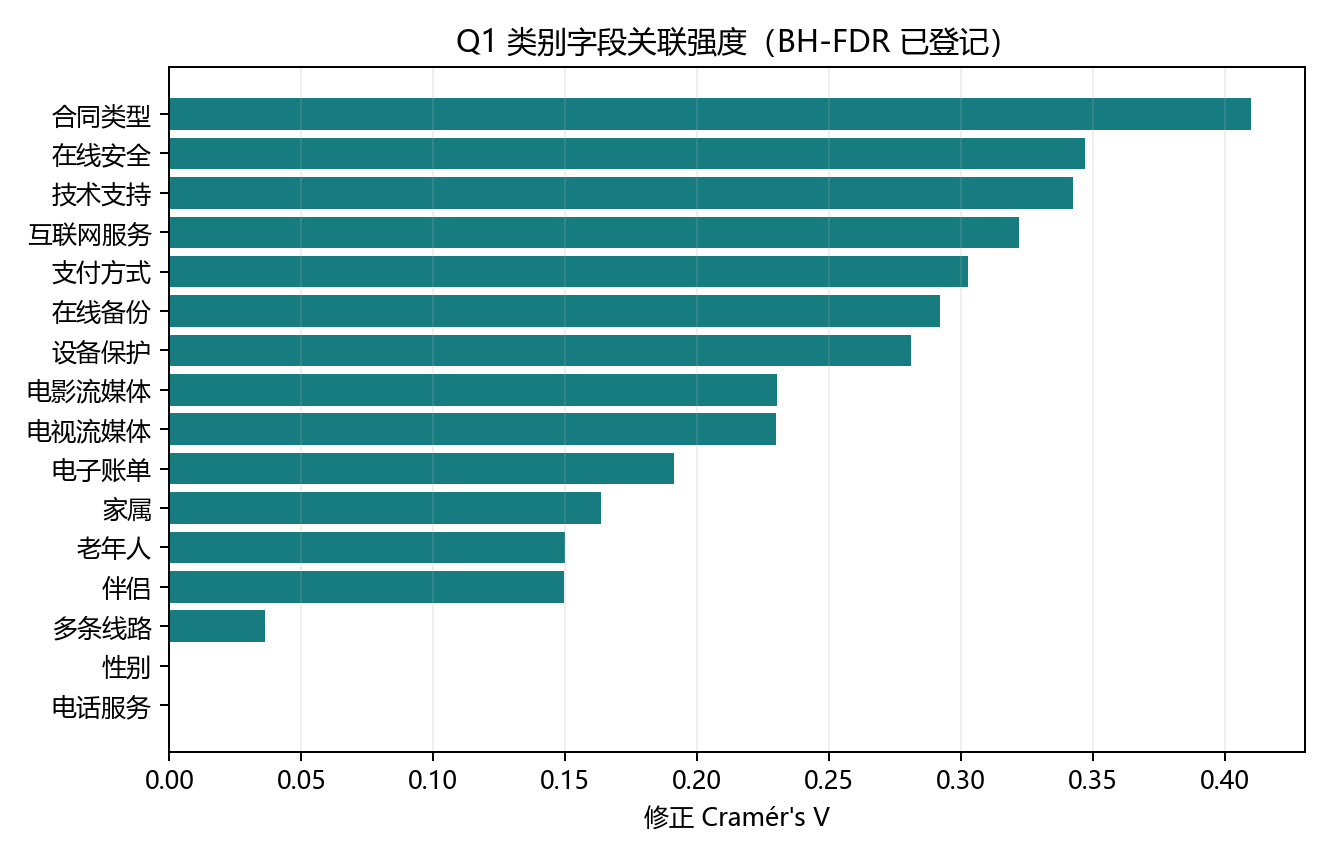
\includegraphics[width=0.88\linewidth]{q1_effect_sizes.png}
\caption{Q1 类别字段的关联效应量；条形排序不表示因果贡献。}
\label{fig:q1-effect-v2}
\end{figure}

\section{Q2：可解释的流失判定方法}
\label{sec:q2-v2}

\subsection{参考类别编码与训练隔离}
令数值特征集合为 \(\mathcal N=\{U,M,T^*\}\)，类别特征集合为 \(\mathcal C\)。对训练折中的数值变量以中位数填补并标准化，对类别变量以训练折众数填补并丢弃参考水平。模型写为
\begin{equation}
z_i=\beta_0+\sum_{j\in\mathcal N}\beta_j\frac{x_{ij}-\widetilde x_j}{s_j}
 +\sum_{j\in\mathcal C}\sum_{\ell\ne\ell_{j0}}\beta_{j\ell}\mathbf 1(x_{ij}=\ell),
\qquad p_i=\sigma(z_i)=\frac{1}{1+e^{-z_i}}.
\label{eq:logistic-v2}
\end{equation}
参数由带 \(L_2\) 正则的对数损失估计：
\begin{equation}
\widehat{\boldsymbol\beta}=\argmin_{\boldsymbol\beta}\left\{-\sum_{i\in\mathcal T}\left[Y_i\log p_i+(1-Y_i)\log(1-p_i)\right]+\frac{\lambda}{2}\lVert\boldsymbol\beta\rVert_2^2\right\}.
\label{eq:logistic-fit-v2}
\end{equation}
每个 OOF 概率都由不含该客户的训练折生成；预处理器也只在训练折拟合。多数类基线和“仅题面核心字段”的 Logistic 用来回答“复杂度是否真的带来增益”，而不是为了制造更多模型名称。

\subsection{隔离评估结果}
固定 20\% 分层留出集含 1409 人；重复 OOF 为 3 次、每次 5 折，所有 7043 人均得到概率。全画像模型相对于核心字段模型的 OOF ROC-AUC 提升约 0.0093，且没有 OOF 缺失。

\begin{table}[H]
\centering
\caption{判定模型的隔离指标}
\label{tab:q2-metrics-v2}
\scriptsize
\begin{tabular}{@{}lrrrr@{}}
\toprule
模型/数据&ROC-AUC&AP&Brier&Log loss\\
\midrule
多数类基线（全体）&0.5000&0.2654&0.1949&0.5786\\
核心字段 Logistic（3x5 OOF）&0.8359&0.6348&0.1398&0.4273\\
全画像 Logistic（3x5 OOF）&0.8451&0.6531&0.1355&0.4174\\
全画像 Logistic（留出集）&0.8422&0.6349&0.1380&0.4203\\
\bottomrule
\end{tabular}
\begin{tablenotes}
\footnotesize\item 注：OOF 折次 AUC 均值为 0.8451、标准差 0.0116；留出集未用于阈值调参。
\end{tablenotes}
\end{table}

500 次 bootstrap 对全画像 OOF 指标给出：ROC-AUC 95\% 区间 [0.8353,0.8551]，\\
AP [0.6280,0.6774]，Brier [0.1313,0.1403]，Log loss [0.4054,0.4298]。

固定等宽箱 ECE 为 0.0130，但最高风险稀疏箱的最大绝对偏差为 0.1068；按分位数分箱后 ECE 为 0.0127、最大偏差为 0.0456。故模型适合排序和分层，不应被描述为“所有风险段都完美校准”。

\begin{figure}[H]
\centering
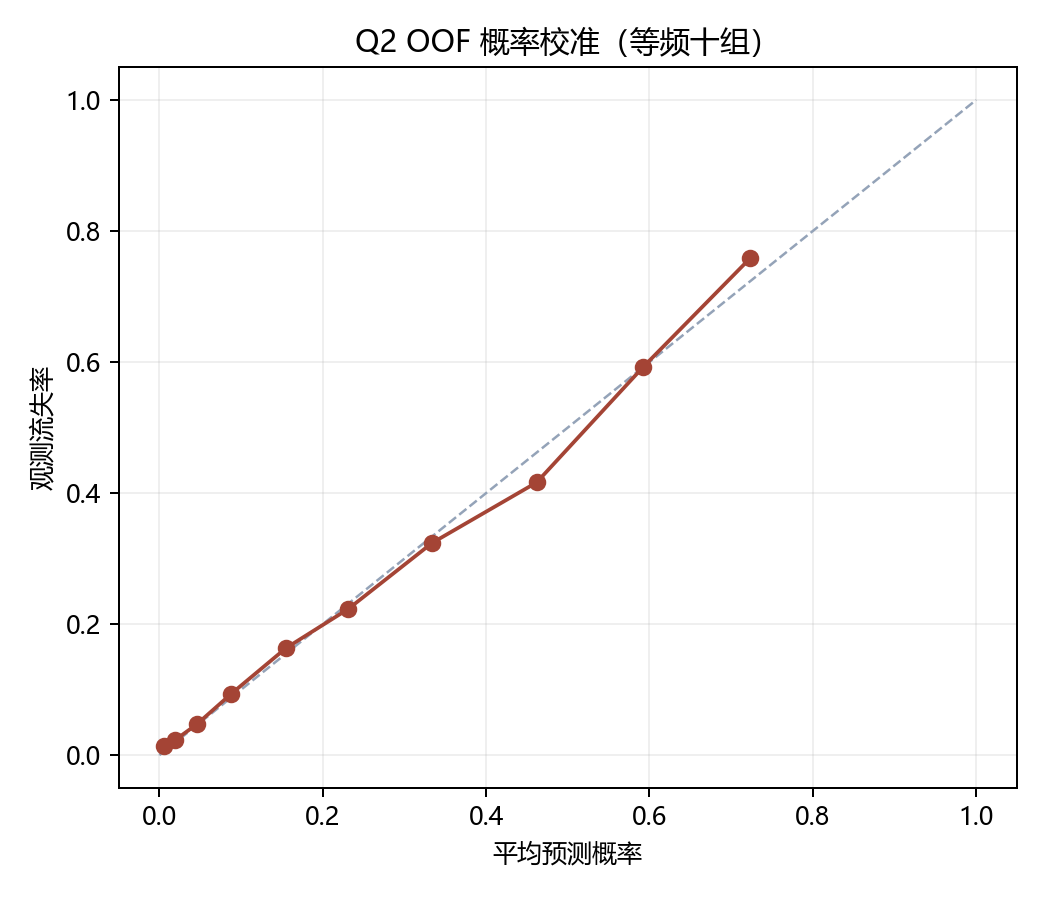
\includegraphics[width=0.83\linewidth]{q2_calibration.png}
\caption{OOF 概率的固定箱与分位数校准；稀疏高风险箱需在新窗口复校准。}
\label{fig:q2-cal-v2}
\end{figure}

\subsection{缺失处理消融与判定接口}
将 11 条结构性空值按 0 月规则处理，与“改用训练折中位数”进行 2 次重复 5 折对照：ROC-AUC 分别为 0.84586 和 0.84574，差异约 \(1.16\times10^{-4}\)，说明本题结果不是由这 11 条记录的单一填补选择驱动。部署接口输出 \(p_i\)、主要触发画像、参考水平、数据窗口和未知类别标记；若未来校准或时间漂移失败，回退到保守基线，不自动扩大覆盖率。

\section{Q3：挽留策略与资源分配}
\label{sec:q3-v2}

\subsection{期望净收益与阈值}
对客户 \(i\) 干预一次，成本为 \(C\)。若不干预时流失概率为 \(p_i\)，对“将要流失客户”的平均挽留成功率为 \(q\)，单个流失损失为 \(L\)，则
\begin{equation}
g_i=p_iqL-C,
\qquad B(S)=\sum_{i\in S}g_i.
\label{eq:net-v2}
\end{equation}
当没有容量约束时，目标对客户可分离，因此
\begin{equation}
g_i\ge0\Longleftrightarrow p_i\ge\tau,
\qquad \tau=\frac{C}{qL}=\frac{150}{0.35\times2000}=0.2142857.
\label{eq:threshold-v2}
\end{equation}
若每天只能处理 \(K\) 人，则把 \(g_i\) 降序排列取前 \(K\) 人。交换论证为：若集合内有 \(g_a<g_b\) 且 \(a\) 入选、\(b\) 未入选，以 \(b\) 替换 \(a\) 后目标增加 \(g_b-g_a>0\)，故排序截断是容量约束下的最优选择。

\subsection{策略比较与独立复算}
表~\ref{tab:q3-policy-v2} 使用同一组 OOF 概率，避免用训练内预测高估收益。阈值策略选择 3281 人（46.59\%），选中组观测流失率 48.19\%，期望净收益为 628279.04 元；全员干预虽然避免损失更高，但因成本覆盖过宽，净收益只有 251786.63 元。

\begin{table}[H]
\centering
\caption{OOF 概率下的挽留策略比较}
\label{tab:q3-policy-v2}
\scriptsize
\setlength{\tabcolsep}{3pt}
\begin{tabular}{@{}lrrrrr@{}}
\toprule
策略&人数&覆盖率&选中组流失率&干预成本/元&期望净收益/元\\
\midrule
不干预&0&0.00\%&--&0&0.00\\
全员干预&7043&100.00\%&26.54\%&1056450&251786.63\\
经济阈值 \(p\ge0.2143\)&3281&46.59\%&48.19\%&492150&628279.04\\
风险排序前 1\%&70&0.99\%&84.29\%&10500&29134.78\\
风险排序前 5\%&352&5.00\%&80.97\%&52800&134611.53\\
风险排序前 10\%&704&10.00\%&75.85\%&105600&250862.17\\
风险排序前 20\%&1408&19.99\%&67.54\%&211200&437095.34\\
风险排序前 30\%&2112&29.99\%&58.90\%&316800&559067.74\\
\bottomrule
\end{tabular}
\begin{tablenotes}
\footnotesize\item 注：期望净收益为 \(\sum_{i\in S}p_iqL-|S|C\)；观测流失率是描述性校验，不是挽留成功率或因果 uplift。
\end{tablenotes}
\end{table}

阈值、人数和收益由第二个实现按
\begin{equation}
\widetilde B(S)=\left(\sum_{i\in S}p_i\right)qL-|S|C
\label{eq:independent-check-v2}
\end{equation}
重新计算，得到选中人数 3281、收益 628279.0392677824 元，与主流程 628279.0392677826 元相差 \(2\times10^{-10}\) 元。500 次行 bootstrap 的阈值策略净收益 95\% 区间为 [608542.74,651432.43] 元；若容量仅允许前 10\% 或前 20\%，区间分别为 [233452.78,268913.39] 和 [415523.46,456602.94] 元。

\begin{figure}[H]
\centering
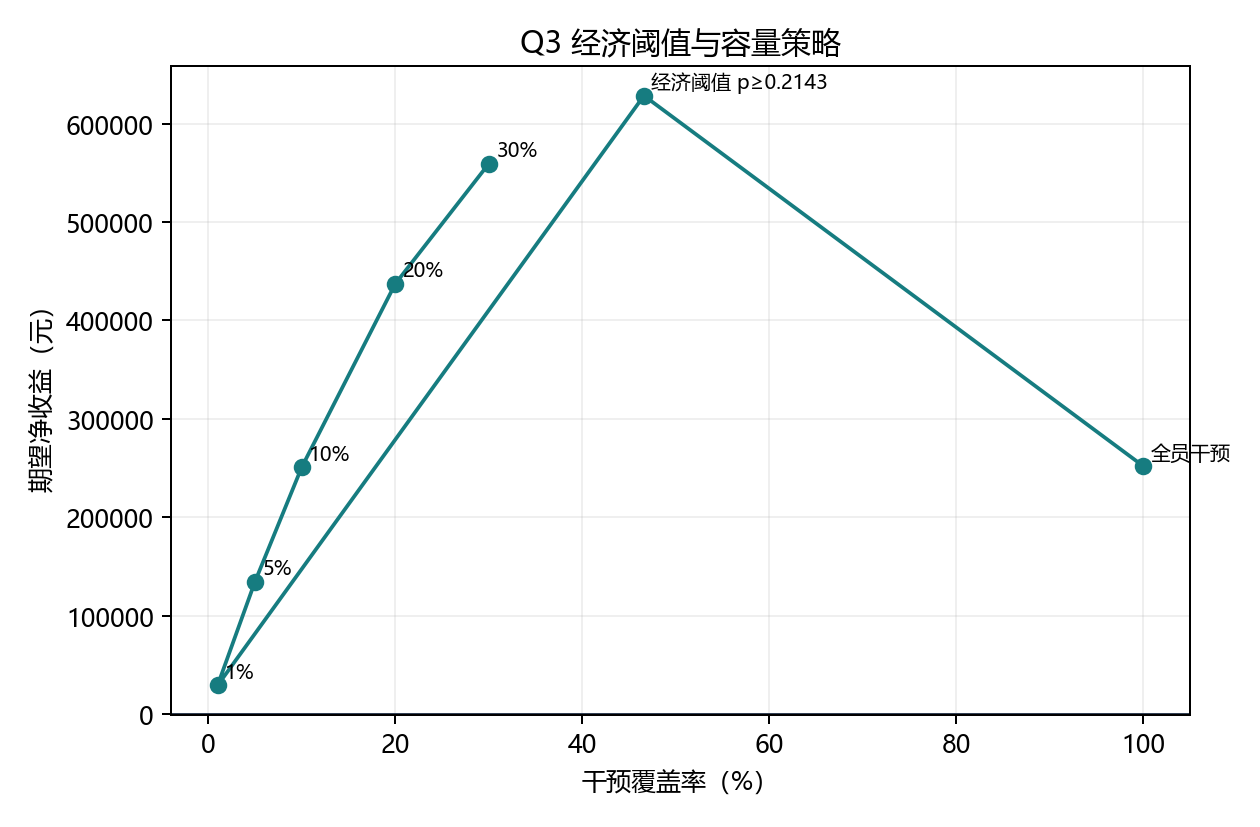
\includegraphics[width=0.88\linewidth]{q3_policy_curve.png}
\caption{固定容量与经济阈值策略的期望净收益曲线；金额是题面参数下的决策值。}
\label{fig:q3-policy-v2}
\end{figure}

\subsection{运营分层}
实际执行采用两层门：先用 \(p_i\ge\tau\) 排除期望净收益为负的客户，再按容量和 \(g_i\) 排序；在同一收益层内，优先核查 Q1 画像中的合同解释、光纤体验、电子支票支付摩擦和短在网服务缺口。话术、优惠强度和触达方式不能由相关模型直接决定，必须通过随机挽留实验估计分层 \(q\) 或 uplift。

\section{Q4：外部冲击下的稳健策略}
\label{sec:q4-v2}

\subsection{显式压力集合}
附件没有竞争价格、宏观指标和时间序列，无法识别外部冲击系数。为回答“如何调整”而不伪造事实，令情景 \(s\) 对基础 log-odds 施加扰动：
\begin{equation}
p_i^{(s)}=\sigma\left(\logit(p_i)+\delta_i^{(s)}\right),
\qquad \logit(p)=\log\frac{p}{1-p}.
\label{eq:shift-v2}
\end{equation}
压力包的联合范围为：竞争扰动 \(u\in[0,0.5]\)，宏观扰动 \(m\in[0,0.3]\)，成功率 \(q_s\in[0.25,0.35]\)，成本 \(C_s\in[150,180]\)，损失 \(L_s\in[1800,2200]\)。合同乘数分别为月付 1.0、一年 0.5、两年 0.2；在网不足 12 个月再乘 \(0.75+0.25\mathbf1(U_i<12)\)。这些区间均标为假设，不能外推为市场参数。

采用 256 点 Latin hypercube sampling（seed=446）覆盖五个连续维度。代表情景如下：
\begin{table}[H]
\centering
\caption{压力包代表情景（假设性）}
\label{tab:q4-scen-v2}
\scriptsize
\begin{tabular}{@{}lrrrrr@{}}
\toprule
情景&竞争 \(u\)&宏观 \(m\)&\(q_s\)&\(C_s\)/元&正收益人数\\
\midrule
LHS-001&0.458&0.037&0.272&155.23&3547\\
LHS-129&0.135&0.205&0.341&154.25&3566\\
LHS-256&0.323&0.128&0.261&162.83&3303\\
\text{最坏角点}&0&0&0.250&180.00&2105\\
\bottomrule
\end{tabular}
\begin{tablenotes}
\footnotesize\item 注：前三行为 LHS 代表点，末行为声明盒约束下的精确最坏角点；任何一行都不代表真实市场情景。完整参数、预测流失率和收益在 \code{results/q4_stress_envelope.json}。
\end{tablenotes}
\end{table}

\subsection{逐人稳健下界与反例}
情景 \(s\) 下的净收益为 \(g_i^{(s)}=p_i^{(s)}q_sL_s-C_s\)，定义
\begin{equation}
r_i=\min_{s\in\mathcal S}g_i^{(s)},
\qquad S_R=\{i:r_i>0\}.
\label{eq:robust-v2}
\end{equation}
在声明的压力假设内，\(S_R\) 有 2105 人（29.89\%），\(\sum_{i\in S_R}r_i=182898.44\) 元；全体客户最小逐人下界为 -179.44 元，中位数为 -93.32 元。这里的下界同时取 256 个 LHS 点与精确最坏角点，因此不把“未采到角点”误当作稳健性。这个结果比只使用窄情景的历史基线更保守，不能视为“策略收益下降”的矛盾证据，而是联合不确定区间扩大后的安全边界。

最不利参数角点的边界阈值约为 0.4：若只知道一个低于该值的基础风险，在该压力包内不应自动干预。它是一个反例边界，不是市场事实。图~\ref{fig:q4-stress-v2} 展示 LHS 代表点和稳健下界；所有情景结论都必须随区间、seed 和外部数据版本一起解释。

\begin{figure}[H]
\centering
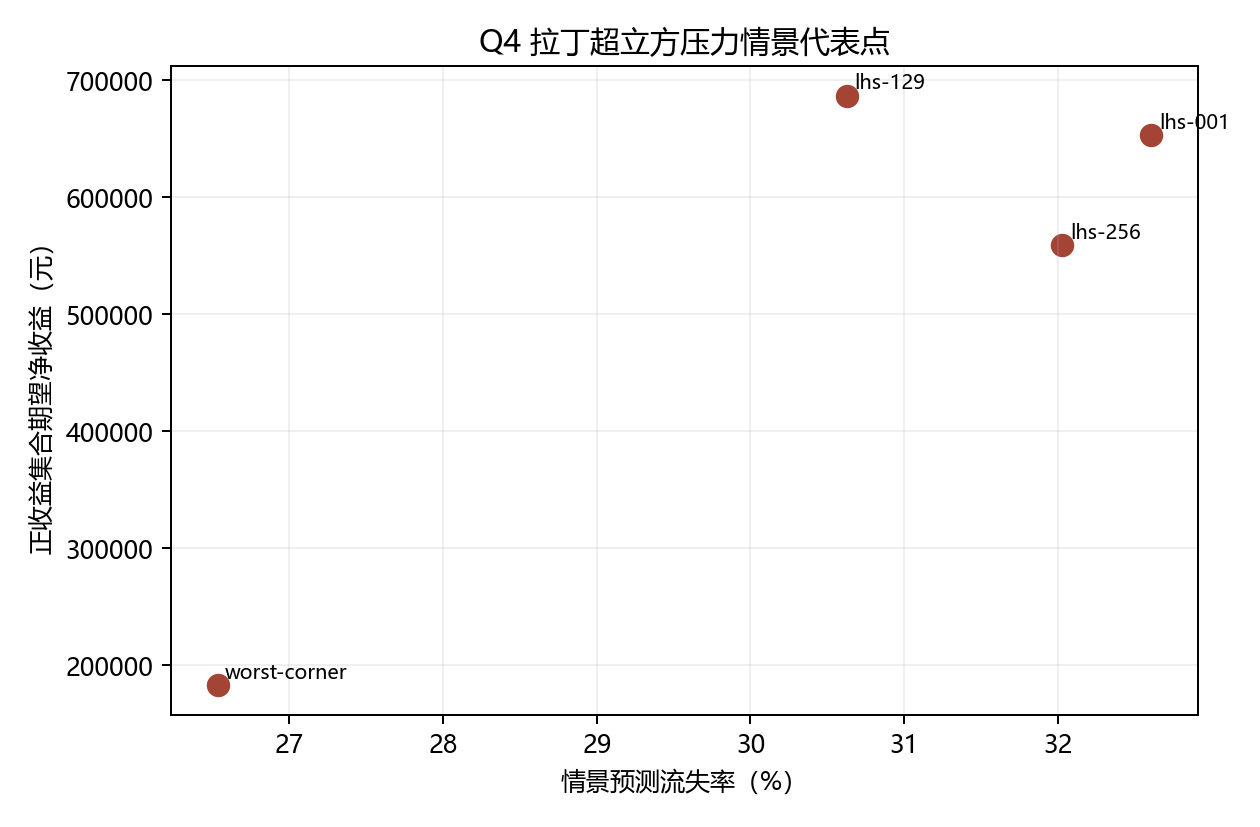
\includegraphics[width=0.88\linewidth]{q4_stress_envelope.png}
\caption{Q4 联合压力包的情景包络与稳健正收益集合。}
\label{fig:q4-stress-v2}
\end{figure}

\subsection{动态调整规则}
\begin{enumerate}[label=\textbf{D\arabic*}.,leftmargin=2.5em]
  \item 每个新标签窗口先检查字段漂移、分层流失率、校准误差和时间切分 AUC；若超过门限，冻结自动扩大覆盖率。
  \item 采集竞争价格、宏观指标、服务工单和触达记录后，重新识别 \(\delta_i^{(s)}\)、\(q_s\)、\(C_s\) 和 \(L_s\)，并保留旧压力包作为回溯基线。
  \item 证据不足时只投放 \(r_i>0\) 的稳健集合；容量不足则按 \(r_i\) 降序截断，并对短在网月付客户人工复核。
  \item 通过随机对照实验记录触达、优惠、续留和成本，逐步把题面平均 \(q\) 替换为可验证的分层效果；实验完成前不把 \(p_i\) 改称为 uplift。
\end{enumerate}

\section{验证、反例与可推广性}
\label{sec:validation-v2}

\subsection{验证矩阵}
本次重跑的证据包将每一关绑定到输入版本 \code{manifest:f262819cfcab8f94d70ac27648b7bdde688d133867760acf47020b9418da7619}、Skill Registry 版本 \code{skill:3d5f0dd4b8bbe91925aca161ff76bb5d5f847516108bcfa1cce91d99dce3bd4e} 和结果摘要哈希 \code{sha256:2d961aee1e60267faf6e184eec7a02397a80c57ff6a63f70399f0bf7d54da858}。关键检查如下：
\begin{table}[H]
\centering
\caption{验证与反例门}
\label{tab:validation-v2}
\scriptsize
\begin{tabularx}{\linewidth}{@{}l l Y l@{}}
\toprule
检查&方法&观察结果&状态\\
\midrule
数据质量&行列、重复、范围、结构性空值&7043/21；重复 0；空值 11 条均可解释&通过\\
Q1 多重比较&\(\chi^2\)+\(V\)+BH&16 个类别字段均保留 \(q\) 值&通过\\
Q2 隔离评估&3x5 OOF + 20\% 留出&OOF AUC 0.8451；留出 AUC 0.8422&通过\\
Q2 不确定性&500 次 bootstrap + 校准&ROC-AUC CI、ECE 和最大偏差均记录&通过\\
缺失消融&结构 0 vs 中位数&11 行改变，AUC 差约 \(1.16\times10^{-4}\)&通过\\
Q3 算术&独立实现式~\eqref{eq:independent-check-v2}&人数一致；收益差 \(<3\times10^{-10}\)&通过\\
Q3 策略不确定性&500 次行 bootstrap&阈值策略 CI [60.85,65.14] 万元&通过\\
Q4 压力&256 点 LHS + 精确角点&稳健集 2105；最坏阈值约 0.4&假设边界\\
\bottomrule
\end{tabularx}
\end{table}

\subsection{不能越过的边界}
\begin{enumerate}[label=\arabic*.,leftmargin=2.5em]
  \item 横截面数据没有时间顺序和随机干预，不能证明合同、价格或服务缺口导致流失；
  \item OOF 只证明当前样本分层重跑的可复现性，不能替代未来月份回测；
  \item \(q=0.35\) 是平均条件成功率，期望净收益不是已实现利润；
  \item Q4 区间未由外部数据校准，稳健下界只对声明的压力集合有效；
  \item 本次“独立复现”是新求解器重跑加 Q3 独立算术，不宣称第二套模型实现；官方格式、匿名、页数和投稿检查仍待 Owner 锁定。
\end{enumerate}

若补充连续月份标签、竞争价格、地区、服务工单和触达结果，可将当前链条升级为时间切分校准、分层 uplift、预算约束多期优化和真实动态压力模型；在此之前，本文输出的是可审计的保守接口。

\section{结论}
\label{sec:conclusion-v2}

针对本题，最稳定的结论不是“某个分类器最好”，而是四个接口共同成立：
\begin{enumerate}[label=\textbf{结论\arabic*}.,leftmargin=2.8em]
  \item 合同类型、在线安全、技术支持、互联网服务和支付方式具有较大的观测关联效应量；在网时长的流失中位数仅 10 个月，而未流失组为 38 个月；
  \item 全画像参考编码 Logistic 的 3x5 OOF ROC-AUC 为 0.8451，留出集为 0.8422，概率适合排序和分层，但稀疏高风险箱需要复校准；
  \item 题面参数导出的经济阈值为 0.2143，OOF 阈值策略选择 3281 人，期望净收益约 62.83 万元，且通过独立算术复核；
  \item 在明确声明的联合压力假设内，2105 人构成逐人最坏收益为正的稳健集合；该数字是安全边界，不是市场预测。
\end{enumerate}

\appendix
\section{复现接口与证据文件}
\label{app:repro-v2}

求解入口为 \code{models/solve_b_problem_v2.py}，完整阶段构建器为 \code{scripts/build_b_replay_artifacts.py}。在仓库根目录执行：
\begin{lstlisting}[language=bash,basicstyle=\ttfamily\small,frame=single,rulecolor=\color{jade},backgroundcolor=\color{papergray},breaklines=true]
python -X utf8 scripts/build_b_replay_artifacts.py ^
  --input-csv "<附件路径>/校赛B题附件.csv" ^
  --input-docx "<题面路径>/校赛B题.docx" ^
  --result-dir runtime/skill-v2-replay/b_solution_v2_final
\end{lstlisting}

阶段证据包括：
\begin{enumerate}[label=\arabic*.,leftmargin=2.5em]
  \item \code{input-manifest.json}：输入哈希、编码、DOCX 结构审计和源资料版本；
  \item \code{problem-contract.json}、\code{question-map.json}、\code{data-contract.json}：题面四问、字段来源、缺失/泄漏门；
  \item \code{derivation-registry.json}：变量、单位、假设、公式和验证引用；
  \item \code{results/summary_v2.json} 及 Q1--Q4 CSV/JSON/PNG：聚合结果，不含客户级风险明细；
  \item \code{validation-report.json}、\code{paper-contract-v2.json}、\code{run-manifest.json}：验证、论文覆盖和运行环境契约。
\end{enumerate}

本次环境记录为 Python 3.9.7、pandas 2.3.3、NumPy 2.0.2、SciPy 1.13.1、scikit-learn 1.4.2、Matplotlib 3.9.4；随机源均记录 seed（42、143、244、345、446）。题面 DOCX 尚未安装 LibreOffice，故只完成结构抽取，未把 DOCX 页面视觉检查误报为通过；本 PDF 自身在 XeLaTeX 双遍编译、\code{pdfinfo}、\code{pdftoppm} 和数学标签审计后再进入发布候选。

\begin{thebibliography}{9}
\bibitem{hosmer} Hosmer, D. W., Lemeshow, S., Sturdivant, R. X. \emph{Applied Logistic Regression}. Wiley, 2013.
\bibitem{benjamini} Benjamini, Y., Hochberg, Y. Controlling the False Discovery Rate. \emph{Journal of the Royal Statistical Society: Series B}, 57(1), 289--300, 1995.
\bibitem{cramer} Cramér, H. \emph{Mathematical Methods of Statistics}. Princeton University Press, 1946.
\bibitem{efron} Efron, B., Tibshirani, R. \emph{An Introduction to the Bootstrap}. Chapman \& Hall, 1993.
\bibitem{sklearn} Pedregosa, F. et al. Scikit-learn: Machine Learning in Python. \emph{Journal of Machine Learning Research}, 12, 2825--2830, 2011.
\end{thebibliography}

\end{document}
